\documentclass{article}%
\usepackage{amsmath}%
\usepackage{amsfonts}%
\usepackage{amssymb}%
\usepackage{graphicx}
\usepackage[shortlabels]{enumitem}
\usepackage{hyperref}

% Custom Font
\usepackage{mathptmx}

% for double figures
\usepackage{caption}
\usepackage{subcaption}

% Appendix Formatting
\usepackage{appendix}
\appendixtitleon % Appendix Title On
\appendixtitletocon % Appendix TOC Title On

% Listings code
\usepackage{listings}
\usepackage{color}

\definecolor{dkgreen}{rgb}{0,0.6,0}
\definecolor{gray}{rgb}{0.5,0.5,0.5}
\definecolor{mauve}{rgb}{0.58,0,0.82}

% enviroment for code
\lstset{frame=tb,
  language=java,
  aboveskip=3mm,
  belowskip=3mm,
  showstringspaces=false,
  columns=flexible,
  basicstyle={\small\ttfamily},
  numbers=none,
  numberstyle=\tiny\color{gray},
  keywordstyle=\color{blue},
  commentstyle=\color{dkgreen},
  stringstyle=\color{mauve},
  breaklines=true,
  breakatwhitespace=true,
  tabsize=3
}

%-------------------------------------------
\newtheorem{theorem}{Theorem}
\newtheorem{acknowledgement}[theorem]{Acknowledgement}
\newtheorem{algorithm}[theorem]{Algorithm}
\newtheorem{axiom}[theorem]{Axiom}
\newtheorem{case}[theorem]{Case}
\newtheorem{claim}[theorem]{Claim}
\newtheorem{conclusion}[theorem]{Conclusion}
\newtheorem{condition}[theorem]{Condition}
\newtheorem{conjecture}[theorem]{Conjecture}
\newtheorem{corollary}[theorem]{Corollary}
\newtheorem{criterion}[theorem]{Criterion}
\newtheorem{definition}[theorem]{Definition}
\newtheorem{example}[theorem]{Example}
\newtheorem{exercise}[theorem]{Exercise}
\newtheorem{lemma}[theorem]{Lemma}
\newtheorem{notation}[theorem]{Notation}
\newtheorem{problem}[theorem]{Problem}
\newtheorem{proposition}[theorem]{Proposition}
\newtheorem{remark}[theorem]{Remark}
\newtheorem{solution}[theorem]{Solution}
\newtheorem{summary}[theorem]{Summary}
\newenvironment{proof}[1][Proof]{\textbf{#1.} }{\ \rule{0.5em}{0.5em}}
\setlength{\textwidth}{7.0in}
\setlength{\oddsidemargin}{-0.35in}
\setlength{\topmargin}{-0.5in}
\setlength{\textheight}{9.0in}
\setlength{\parindent}{0.3in}


%% THEO: Custom Quote Blocks
%\usepackage{showframe,lipsum}
\usepackage[most]{tcolorbox}
\definecolor{block-gray}{gray}{0.85}
\newtcolorbox{myquote}{colback=block-gray,grow to right by=-10mm,grow to left by=-10mm,
boxrule=0pt,boxsep=0pt,breakable}

\begin{document}
\title{UBlox C099-F9P GPS-RTK Demo Setup Instructions}
\author{Theodore Stangebye, Dr. Timothy Mohr\\
Grove City College\\
\texttt{\{stangebyeto1,mohrta\}@gcc.edu}}
\maketitle
%\begin{flushright}
%\textbf{Theo Stangebye}
%\end{flushright}


%\begin{center}
%\textbf{} \\
%\end{center}


%%%%%%%%%%%%%%%%%% START

%\begin{center}
%	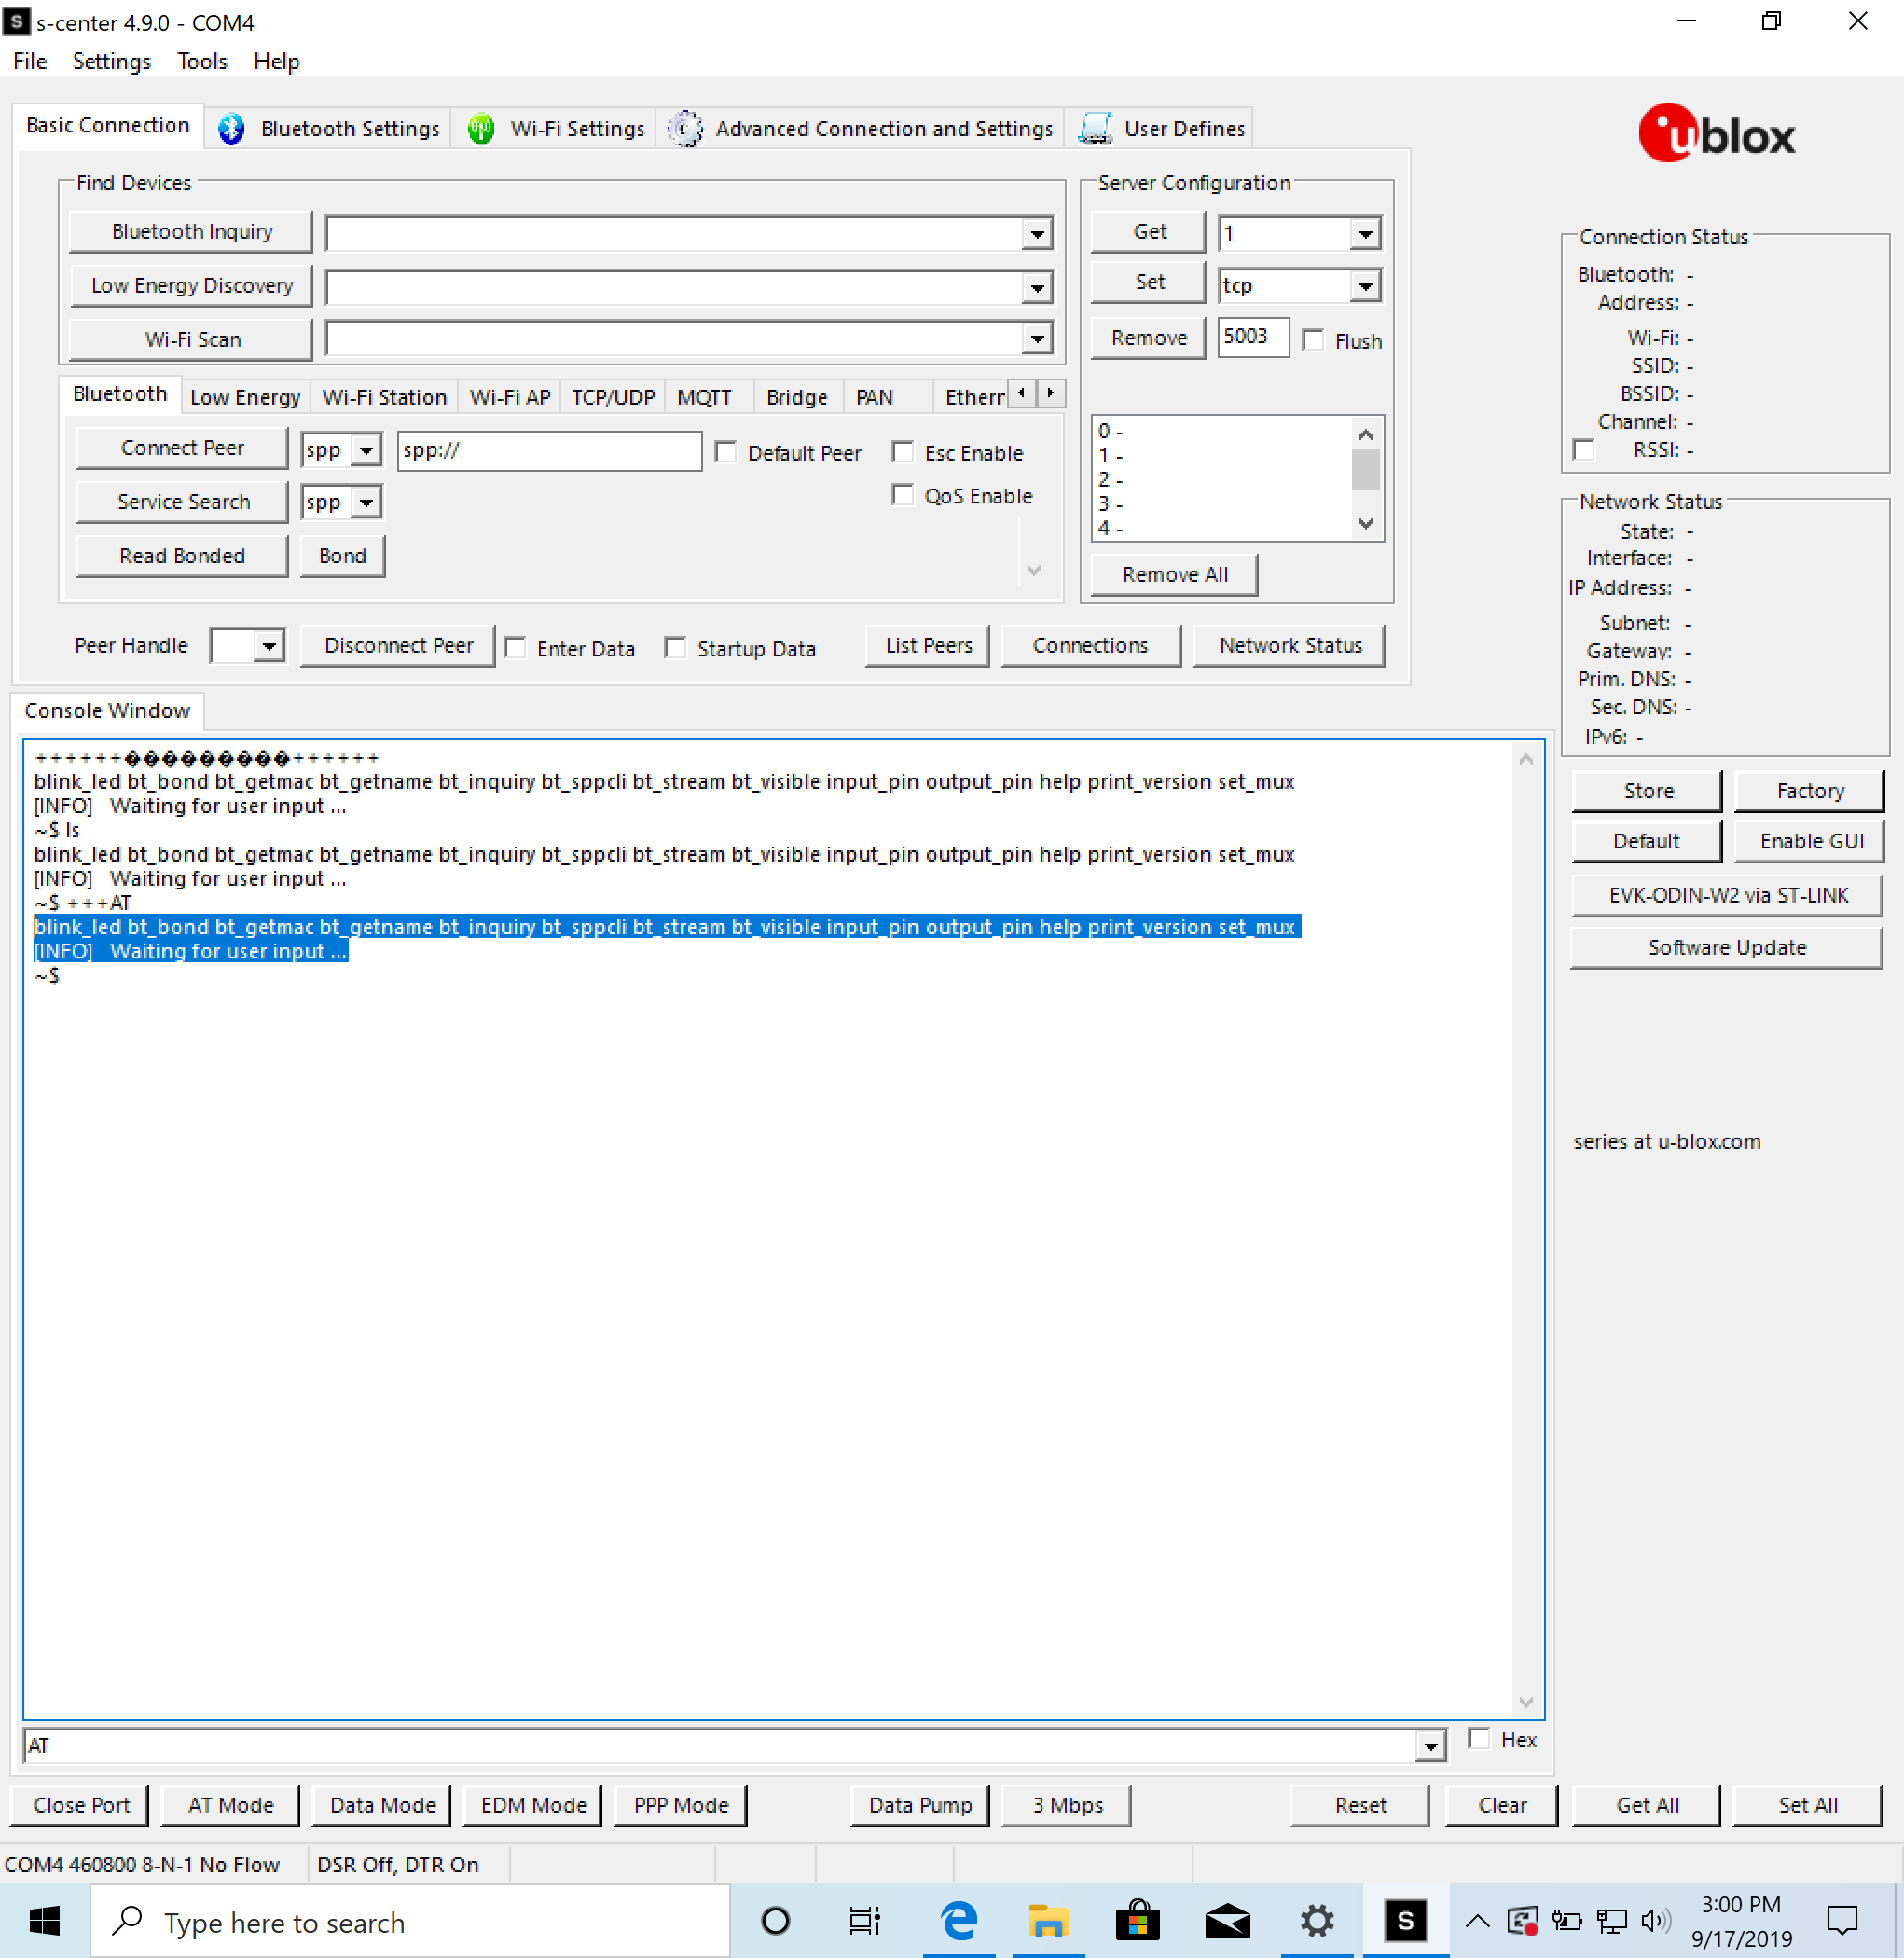
\includegraphics[scale=.5]{./imgs/img0.png}
%\end{center}

% Center table of contents on first page.
\vspace*{\fill}
\tableofcontents
\vspace*{\fill}

\newpage

\section{Introduction}
This document hopes to guide new users through the process of implementing a GPS-RTK demo using two C099-F9P development boards from UBlox. 
This guide draws heavily from the Ublox C099-F9P User Manual, but is laid out linearly, so that new users can walk through the setup process end-to-end.
The guide also gives instructions for updating the firmware of the ODIN-W2 modules, which is not well documented in the user manual and online to our knowledge.

\subsection{References}\label{ref:references}
	\begin{itemize}
		\item C099-F9P User Guide:\\ \href{https://github.com/gcc-ant-robot/gps-rtk/raw/master/documentation/C099-F9P/C099-F9P-AppBoard-ODIN-W2-CSW_UserGuide_(UBX-18055649).pdf}{\texttt{https://github.com/gcc-ant-robot/gps-rtk/raw/master/documentation/C099-F9P/\\C099-F9P-AppBoard-ODIN-W2-CSW\_UserGuide\_(UBX-18055649).pdf}}
		\item GCC GPS-RTK GitHub Repository: \\
		\url{https://github.com/gcc-ant-robot/gps-rtk}
	\end{itemize}

\subsection{Board Components \& Descriptions}
	Each C099-F9P board has two main modules:
	\begin{itemize}
		\item \textbf{F9P GPS Receiver}: This module is the GPS receiver of the board.  It receives RTCM data from an external source and utilizes the GPS antenna to create an RTK solution.  In the case of the Base Station unit, the F9P generates RTCM data which is sent to the rover unit.
		\item \textbf{ODIN-W2 Wifi/Bluetooth Gateway}: this module acts as a radio link, enabling the F9P to receive RTCM data wirelessly over a wifi or bluetooth network.  In the case of the Base Station, the ODIN-W2 receives a data stream of RTCM from its neighboring F9P Module and sends that data stream over the network to the rover unit.
	\end{itemize}

	\begin{myquote}
	Note: only connect one GPS unit to your computer at a time in order to avoid confusing multiple units and writing data to one which you did not intend to write data to!	
	\end{myquote}


\subsection{Preliminary Setup}\label{ref:down_config}
	\begin{enumerate}
		\item Download and unzip (or extract if you're on windows) the configuration folder here: \\ \href{https://gcc-gps-rtk.s3.amazonaws.com/GCC\_Ublox\_GPSRTK\_Config.zip}{\texttt{https://gcc-gps-rtk.s3.amazonaws.com/GCC\_Ublox\_GPSRTK\_Config.zip}}
		\item Make sure you have Ublox S-Center Installed: \\ \href{https://www.u-blox.com/en/product/s-center}{\texttt{https://www.u-blox.com/en/product/s-center}
		\item Make sure you have Ublox U-Connect Installed: \\ \href{https://www.u-blox.com/en/product/u-center}{\texttt{https://www.u-blox.com/en/product/u-center}}}
	\end{enumerate}

\section{Base Station GPS Setup}
\subsection{Base Station Mechanicals}
	\begin{enumerate}
		\item Connect the Wifi and GPS Antennas to the base station board.
		\item Make sure all jumpers are removed from the base station board except the single jumper located next to the battery connector.
		\item Connect the base station GPS receiver to your laptop with a USB cable as shown in Figure \ref{fig:phys}.
	\end{enumerate}
	
%	width=.8\linewidth
	\begin{figure}
	\centering
	\begin{minipage}{.5\textwidth}
	  \centering
	  \includegraphics[height=3in]{./images_for_tutorial/basestationphys.jpeg}
	  \captionof{figure}{Physical Setup of the Base Station GPS Receiver.}
	  \label{fig:phys}
	\end{minipage}%
	\end{figure}
	
%	\begin{center}
%	\includegraphics[width=4in]{./images_for_tutorial/basestationphys.jpeg}
%	\end{center}
	
	\begin{myquote}
		Note, my MacBook Pro does not have USB A ports, and so I am using an inline converter as seen in Figure \ref{fig:phys}. This dongle can be ignored as it is basically a USB passthrough, converting USB-C to USB-A.
	\end{myquote}

\subsection{Reset Base Station ODIN-W2 to Known State}
We need to set the ODIN-W2 to a known state, and so we will flash it with factory firmware to erase any configurations which exist on the module.  See instructions for this operation in Appendix \ref{ref:odin_firmware}.

\subsection{Base Station ODIN-W2 Configuration}
	
	In this section, it is assumed that we have just flashed new firmware to the base station's ODIN W2 module, resetting it to its factory defaults.  We will now load a configuration file to it which will allow it to broadcast correction data from the base-station's F9P GPS receiver over the network to a known IP address (which will be the IP of the rover) . This configuration will also tell the base station to connect to the rover's wifi network (which will be called "UBXWifi").  These instructions correspond to section 6.1 (page 24) of the C099-F9P UserGuide (Linked in Section \ref{ref:references} of this document).
	\begin{enumerate}
	\item Connect to the ODIN-W2 in S-Connect.
	\item In the S-Connect window, click on the File menu and select "Download Configuration".  Then, navigate to the \texttt{Base ODIN-W2 Station UDP client.txt} file within the configuration folder you downloaded during Section \ref{ref:down_config}.  Within the Configuration folder, this text file is located at\\ \texttt{.\textbackslash GCC\_Ublox\_GPSRTK\_Config\textbackslash ublox-C099\_F9P-uCS-master\textbackslash odin-w2\textbackslash Base ODIN-W2 Station UDP client.txt}.
	\item Once this file is selected, click the "Open" button to load these settings onto your ODIN W2 module.
	\item Connect the ODIN to the F9P unit by placing a jumper in position \texttt{30E}. See Figure \ref{fig:3oe}.
	\item Continue with next Section \ref{ref:bs_f9p_config}.
	\end{enumerate}
	
	\begin{figure}
	\centering
	\begin{minipage}{.5\textwidth}
	  \centering
	  \includegraphics[height=3in]{./images_for_tutorial/3oe.jpeg}
	  \captionof{figure}{Jumping the \texttt{3OE} pins to connect the ODIN to the \\\ F9P module.}
	  \label{fig:3oe}
	\end{minipage}%
	\begin{minipage}{.5\textwidth}
	  \centering
	  \includegraphics[height=3in]{./images_for_tutorial/resetdefaults}
	  \captionof{figure}{Reset the F9P module to its default state with this button in U-Center.}
	  \label{fig:resetdefaults}
	\end{minipage}
	\end{figure}
	
\subsection{Base Station F9P Configuration}\label{ref:bs_f9p_config}
	In this section, we tell the base station's GPS receiver (F9P) to stream RTCM data to the ODIN, which has just been configured to receive this data in the last section.  We deviate from the C099-F9P user guide's instructions on this operation (which are given in section 6.1.3.1 of the C099-F9P user guide) so that the base station will automatically begin's its survey-in operation when power is connected.
	
	\begin{enumerate}
	\item Open U-Center
	\item Connecting to the GPS Receiver: in the "Receiver" window menu of U-Connect, select "Connection $\rightarrow$ COM15".  Remember to replace "COM15" with the address of your GPS unit.
	
	\begin{myquote} Note: this com port will not be the same com port which you used to communicate with your ODIN module. There is a USB multiplexor on the GPS development board, which has multiple virtual COM ports for the different on-board devices.  From previous experience, the COM port of the GPS receiver which you should use with the U-Center software tends to be the highest COM number which appears.  When connected to the GPS receiver, you'll see that the instrument fields will begin to show live GPS data as seen in Figure \ref{fig:livedata}.
	\end{myquote}
	
	\begin{figure}
		\centering
		\includegraphics[width=.8\textwidth]{./images_for_tutorial/livedata.png}
		\captionof{figure}{Live Data from GPS unit shown in U-Center.}
		\label{fig:livedata}
	\end{figure}
	
	\item Reset the GPS receiver to its default settings, as seen in Figure \ref{fig:resetdefaults}.
	
	As shown in \textbf{Section 6.1.3.1 of the C099-F9P user manual}, load the base station's F9P configuration file into the GPS units memory:
	
	\begin{enumerate}
	
	\item In the View menu, select "Generation 9 Configuration View"
	\item Select the "Advanced Configuration" sidebar item in the Generation 9 Configuration View window.
	\item Click the "Load" Button on the right-hand side of the screen.
	\item Select the "\texttt{F9P Base config C99.txt}" file from the configuration folder you downloaded in Section \ref{ref:down_config} and click "Send".  Note, this configuration file is at\\ \texttt{.\textbackslash GCC\_Ublox\_GPSRTK\_Config\textbackslash ublox-C099\_F9P-uCS-master\textbackslash zed-f9p\textbackslash F9P Base config C99.txt} within the configurations folder.
	\item Once the \texttt{F9P Base config C99.txt} file has been selected and is loaded into UBlox, click the "Send" button and check that each line of the configuration has a check mark.  See below video note for assistance.
	
	\end{enumerate}
	
	\begin{myquote}
		A \textbf{video} showing steps a-e is located at 	\url{https://youtu.be/qwOFgIJDMoE}.
	\end{myquote}

	\begin{myquote}
		Note: if you want the base station to use a fixed location (bypassing the base station's survey-in feature), you should not complete step \ref{ref:set_SVIN} here.]\\  
		The survey-in (SVIN) feature configures the base station to empirically estimate its location at startup. (The location of the base station has great impacts on the absolute accuracy of the rover's location solution. \\
		If an accurate location of the base station is known, hard-coding this location into the base station is desirable.  This way, our rover's location solutions will not rely on the assumption that the base station was able to accurately estimate its location at startup through the survey-in process.
	\end{myquote}

	\item The settings which have just been uploaded to the board setup the pipeline for sending RTCM correction data.  However, no data will flow from the F9P to the ODIN until we enable the Survey\_In functionality of the base station. For this reason, we enter the following settings:
	
		\begin{myquote}
			A \textbf{video} showing steps a-e is located at \url{https://youtu.be/F4EOG5IoqP4}.
		\end{myquote}
		
	\begin{enumerate}\label{ref:set_SVIN}
		\item In the left scroll portion of the window, scroll down and expand the \texttt{CFG-TMODE} section.
		\item Select the \texttt{CFG-TMODE-MODE} option, and then use the "Modify" tool on the right hand side of the window to set the value to \texttt{1} for \texttt{SURVEY\_IN}, and add this to the \texttt{flash} layer so that this change will be stored in non-volatile memory.  (To add these configurations to the flash layer, click the "set in flash" button.  This option enables the base station's Survey In feature, which allows the base station to determine its own reference point from which it will derive GPS errors and subsequent correction information.
		\item Now select the \texttt{CFG-TMODE-SVIN\_MIN\_DUR} and set its value to \texttt{60} and add this to the flash layer as well.  This tells the base station to wait at least 60 seconds before beginning to send correction data.  
		\item Now select the \texttt{CFG-TMODE-SVIN\_ACC\_LIMIT} and set its value to \texttt{50000}.  Add this to the flash layer as well.  This sets threshold on the GPS location standard deviation which must be met before correction data will be sent to the rover.
		\item Remember to press the SEND button before closing this window to upload these settings to the GPS receiver!
		\newline
		\newline
		To recap steps 10-12, we updated the following settings:
		\begin{lstlisting}
		Flash CFG-TMODE-MODE       1.               # write value 1 - SURVEY_IN
		Flash CFG-TMODE-SVIN_MIN_DUR 0x3c           # write value 60  0x3c     
		Flash CFG-TMODE-SVIN_ACC_LIMIT 0xc350.      # write value 50000  0xc350
		\end{lstlisting}

	\end{enumerate}

	\item Unplug the Base Station GPS unit from your laptop.

	\end{enumerate}
	The GPS Receiver Base Station should now be good to go!\\
	
	\begin{myquote}
	\textbf{How to check the Base Station's Survey In Status:} You can check that your configuration changes to the Base Station's F9P unit have been successful by going to "View $\rightarrow$ Messages View" in the U-Center window menu, and then using the left sidebar to view the \texttt{UBX-NAV-SVIN} message.  In Figure \ref{fig:svin}, we can see that the Survey In process has begun but that even though it's been running for almost 400 seconds, its solution is not valid because the mean standard deviation of the GPS solutions is almost 30 meters, which is above the threshold we set in step 12. 
	\end{myquote}

	\begin{figure}
		\centering
		\includegraphics[width=.8\textwidth]{./images_for_tutorial/svin}
		\captionof{figure}{Survey In Message Shown in Messages View.}
		\label{fig:svin}
	\end{figure}

\section{Rover GPS Setup}
\subsection{Rover Mechanicals}
	\begin{enumerate}
		\item Connect the Wifi and GPS Antennas to the rover board.
		\item Make sure all jumpers are removed from the rover board except the single jumper located next to the battery connector.
		\item Connect the rover GPS receiver to your laptop with a USB cable as shown in Figure \ref{fig:phys}.
	\end{enumerate}

\subsection{Reset Rover ODIN-W2 to a Known State}
Please see Appendix \ref{ref:odin_firmware} for instructions on resetting the ODIN-W2 module to factory settings through a firmware update.

\subsection{Rover ODIN-W2 Configuration}
In this section, we have just flashed new firmware to the rover's ODIN-W2 module, resetting it to its factory defaults.  We will now load a configuration file to it which will allow it to receive correction data from the base station.  This section will also setup the rover GPS development board to put out its own WiFi network, to which the base station will connect.

Begin with the rover GPS development board plugged into your laptop with a USB cable.

\begin{enumerate}
\item Open S-Center and connect to the rover with the settings shown in Figure \ref{fig:s-centerconnection}, replacing \texttt{COM8} with the COM port of your rover's ODIN module. Note: you may need to use the "Refresh COM Ports" button if you do not see a COM port for your ODIN module.
\item In the "File" menu of the S-Center window, click "Download Configuration" and navigate to the \texttt{Rover ODIN-W2 Access Point UDP Server.txt} file within the configuration folder you downloaded in Section \ref{ref:down_config}.

	Within the Configuration folder, this text file is located at \\ \texttt{.\textbackslash GCC\_Ublox\_GPSRTK\_Config\textbackslash ublox-C099\_F9P-uCS-master\textbackslash odin-w2\textbackslash Rover ODIN-W2 Access Point UDP Server.txt}.
\item Once this file is selected, click the "Open" button to load these settings onto your ODIN W2 module.
\item Connect the ODIN to the F9P unit by placing a jumper in position \texttt{30E}. See Figure \ref{fig:3oe}.
\item Reboot the GPS board by either pressing the RESET button or disconnecting and reconnecting its USB cable.
\item You'll know that you performed this section correctly when you see a "UBXWifi" wifi network appear.
\item Continue with Section \ref{ref:Rover_f9p_config}.
\end{enumerate}

\subsection{Rover F9P Configuration}\label{ref:Rover_f9p_config}

In this step, we configure the Rover GPS development board's F9P module to receive RTCM corrections from the rover's ODIN-W2 Module.

\begin{enumerate}
 
	\item Begin with the rover's GPS development board connected to your laptop over USB.
	\item Open U-Center and connect to the Rover GPS unit by selecting "Receiver $\rightarrow$ COM15", replacing "COM15" with the COM port of your board. (remember that you may have to try several COM ports and see which one spits out GPS data.)
	\item Reset the GPS Receiver by clicking the button shown in Figure \ref{fig:resetdefaults}.
	\item In the View menu, select "Generation 9 Configuration View"
	\item Select the "Advanced Configuration" sidebar item in the Generation 9 Configuration View window.
	\item Click the "Load" Button on the right hand side of the screen.
	\item Select the \texttt{F9P Rover config C99.txt} file from the configuration folder you downloaded in Section \ref{ref:down_config} and click "Send".  Note, this configuration file is at \\ \texttt{.\textbackslash GCC\_Ublox\_GPSRTK\_Config\textbackslash ublox-C099\_F9P-uCS-master\textbackslash zed-f9p\textbackslash F9P Rover config C99.txt} within the configurations folder.
	\item Restart the rover GPS by pressing the RESET button.
\end{enumerate}

\section{Test}
\begin{enumerate}
	\item Go outside, plug the Base station into a battery pack.  Give it several minutes to survey in.
	\item Take your laptop and use U-Connect to connect to the rover GPS unit.  See if you can get a \texttt{DGNSS/RTK/Fixed} Solution!
\end{enumerate}

%\appendix
\begin{appendices}


\section{ODIN-W2 Firmware Upgrade}\label{ref:odin_firmware}
	When receiving a new GPS unit, the firmware on the ODIN-W2 (also known as ODIN) will likely need to be updated.  This process is shown below and draws from Section 7.2 of the C099-F9P user guide which is linked in Section \ref{ref:references} of this document.  Note that the files, which the manual instructs users to download, are already contained in the configuration folder which was downloaded in section \ref{ref:down_config} of this document (ie. If you downloaded the folder on page 1 of this document, you don't have to download any other configuration files).
	
	\begin{myquote}
	Note: an external power source may be required for the GPS board if the firmware update causes the board to repeatedly power cycle.	(more to come on this).
	\end{myquote}

	
	\begin{enumerate}
	\item Open the S-Center app on your Windows Laptop.  If S-Center is already open, click the "Open Port" button to open the connection window seen in Figure \ref{fig:com4show}.
	\item Click "Refresh COM Ports".  Note which port corresponds to the device name ending in "ODIN-W2".  For me, this is \texttt{COM4}, as seen in Figure \ref{fig:com4show}.
	\item Place a jumper over the \texttt{SB ODIN} pins (pin pair closest to the Large RGB LED on your development board as seen in Figure \ref{fig:sb}).  This jumper will enable the ODIN's safeboot mode during next startup.
	\item Now, restart the development board by either unplugging the USB cable 
	\item from your laptop and reconnecting it, or by pressing the "RESET" button on the development board (button closest to the GPS connector on the board).
	\begin{figure}
	  \centering
	  \includegraphics[height=3in]{./images_for_tutorial/com4show.png}
	  \captionof{figure}{Observing the COM port of the ODIN Module in S-Center.}
	  \label{fig:com4show}
	\end{figure}
	
	\item The ODIN is now in safe-boot mode, and is ready to have a new firmware version flashed to its memory.
	\item In File Explorer, navigate into the configuration folder which you downloaded in Section \ref{ref:down_config}.  I extracted my folder to my Downloads Folder, so I navigate to \texttt{\textbackslash Mac\textbackslash Home\textbackslash Downloads\textbackslash GCC\_Ublox\_GPSRTK\_Config\textbackslash }
	\item Now, within this folder, go to the \texttt{ODIN-W26X-7} directory which should be at\\ \texttt{.GCC\_Ublox\_GPSRTK\_Config\textbackslash ODIN-W26X-7\textbackslash }.
	
	
	\begin{figure}
	\centering
	\begin{minipage}{.5\textwidth}
	  \centering
	  \includegraphics[height=3in]{./images_for_tutorial/sb}
	  \captionof{figure}{Safe-boot enabled by jumping pins \texttt{SB ODIN}.}
	  \label{fig:sb}
	\end{minipage}%
	\begin{minipage}{.5\textwidth}
	  \centering
	  \includegraphics[width=\textwidth]{./images_for_tutorial/wxfolder.png}
	  \captionof{figure}{Root directory of the configuration folder downloaded in Section \ref{ref:down_config}.}
	  \label{fig:wxfolder}
	\end{minipage}
	\end{figure}
	
		You should see the files shown in Figure \ref{fig:wxfolder}.
	\item In File Explorer's "File" menu, click on "Open Windows PowerShell", this will give you a PowerShell terminal inside the \texttt{ODIN-W26X-7} folder.
	\item Flash the boot-loader by pasting the following into the Powershell window, replacing \texttt{COM4} with your own COM port. See Figure \ref{fig:bootload}.
	\begin{lstlisting}[language=bash]
		.\stm32flash.exe -b 115200 -w '.\Bootloader - only needed for recovery\ODIN-W2-BOOT-v0.8.2.bin' -s 0x8000000 COM4
	\end{lstlisting}
	
	\item Now, flash the firmware update to the ODIN by pasting the following command, again replacing \texttt{COM4} with the COM port for your ODIN.  Note that this command should take several minutes to run successfully, but you'll know that it's working if you see something akin to Figure \ref{fig:odinfirm}.

	\begin{lstlisting}[language=bash]
		.\stm32flash.exe -b 115200 -w .\ODIN-W26X-SW-7.1.0-020.bin -S 0x8010000 COM4
	\end{lstlisting}
	
	\begin{figure}
	\centering
	\begin{minipage}{.5\textwidth}
	  \centering
	  \includegraphics[width=\textwidth]{./images_for_tutorial/bootload}
	  \captionof{figure}{Erasing the configurations on an ODIN module.}
	  \label{fig:bootload}
	\end{minipage}%
	\begin{minipage}{.5\textwidth}
	  \centering
	  \includegraphics[width=\textwidth]{./images_for_tutorial/odinfirm}
	  \captionof{figure}{Flashing new configs to an ODIN module.}
	  \label{fig:odinfirm}
	\end{minipage}
	\end{figure}
	
	\item When the previous step is complete, remove the \texttt{SB ODIN} jumper and then restart the GPS receiver by either pressing the RESET button or unplugging/plugging the USB cable back into your laptop.
	\item We will now test the ODIN's firmware upgrade by attempting to connect to it with S-Center.
	\item Go back to the S-Center App, you will now connect to the ODIN with the settings showing in Figure \ref{fig:s-centerconnection} by clicking "Open Port".  Remember to replace \texttt{COM4} with the COM address associated with your ODIN module.
	\item Before entering any data on the ODIN module through the s-center interface, click the "EVK-ODIN-W2 via ST-LINK" button shown in Figure \ref{fig:evk}.
	\item Verify that you have a working connection to the ODIN by clicking the "AT Mode" button.  You should see some text flash through the console ending with "OK".

	Before we finish, we need to update the ODIN's Baud rate so that it matches the F9P's Baud rate.  If this step is forgotten, the two modules will not be able to communicate with each other.
	\item Change to the "User Defines" tab in S-Center.  Enter and run the following commands sequentially.  These commands change the baud rate of the ODIN to \texttt{460800} Baud, write the configuration to memory, and then restart the unit.  This is necessary (in my understanding) because the GPS receiver communicates at \texttt{460800} Baud.
		\begin{lstlisting}
		AT+UMRS=460800,2,8,1,1,0
		AT&W
		AT+CPWROFF
		\end{lstlisting}
		
		
			\begin{figure}
			\centering
			\begin{minipage}{.5\textwidth}
			  \centering
			  \includegraphics[width=\textwidth]{./images_for_tutorial/s-centerconnection}
			  \captionof{figure}{S-Center Connection Configuration.}
			  \label{fig:s-centerconnection}
			\end{minipage}%
			\begin{minipage}{.5\textwidth}
			  \centering
			  \includegraphics[width=\textwidth]{./images_for_tutorial/evk}
			  \captionof{figure}{EVK-ODIN-W2 via ST-LINK button encircled.}
			  \label{fig:evk}
			\end{minipage}
			\end{figure}
		
		The output of running these commands should look something like this in the terminal. We will have to reconnect to the ODIN module at \texttt{460800} Baud.
		\begin{lstlisting}
		AT+UMRS=460800,2,8,1,1,0
		OK
		AT&W
		OK
		AT+CPWROFF
		OK
		??
		\end{lstlisting}
	
		\item Click "Close Port" in the S-Center Window.
		\item Now click "Open Port" in the S-Center Window to bring up the connection configuration page.  We will keep the same settings as we used before (Figure \ref{fig:s-centerconnection}), except change the Baud rate to \texttt{460800}.  Connect to the ODIN.  If you see the AT console spit out readable messages, then congratulations! You may now continue with the instructions which directed you here.
	
	\end{enumerate}
	
	\section{List of Terms}

\begin{itemize}
	\item RTCM: Correction data which is sent from the GPS Base station to the Rover Module in order to improve the accuracy of the Rover's location solution.
	\item GPS-RTK: Global Positioning System Real Time Kinematics.
	\item Rover: GPS module mounted on moving "roving" robot.
	\item Base Station: GPS module permanently fixed in a specific location.  Provides correction data to Rover.
\end{itemize}

\end{appendices}

\end{document}